\documentclass[letterpaper,12pt]{article}
% reduce margins
\usepackage[margin=0.5in]{geometry}
% remove indent
\setlength\parindent{0pt}
\setlength{\parskip}{1em}
% reduce toc spacing
\usepackage{tocloft}
\setlength{\cftbeforesecskip}{0.5em}
% make toc show subsubsections
\setcounter{tocdepth}{3}
% remove section numbering
\setcounter{secnumdepth}{1}

% reduce section, subsection, etc spacing
\usepackage{titlesec}
\titlespacing*{\section}{0pt}{0\baselineskip}{0\baselineskip}
\titlespacing*{\subsection}{0pt}{0\baselineskip}{0\baselineskip}
\titlespacing*{\subsubsection}{0pt}{0\baselineskip}{0\baselineskip}

%reduce list spacing
\usepackage{enumitem}
\setlist{nosep}

\usepackage[hidelinks]{hyperref}

\usepackage[backend=biber]{biblatex}
\addbibresource{references.bib}

\usepackage{graphicx}

\title{Lab 2 - Linguistics Data, Stat 215A, Fall 2024\vspace{-2em}}

\begin{document}
\maketitle

These are the \textbf{lab2-specific} instructions. Please also see the general lab instructions in \textbf{lab-instructions.pdf}.

\tableofcontents

\section{Submission}
Push a folder called \texttt{lab2} to your \texttt{stat-215-a GitHub} repository by 23:59 on Friday, October 4th. I will run a script that will pull from each of your GitHub repositories promptly at midnight so take care not to be late as late labs will not be accepted.

\textbf{Follow the general lab instructions in stat-215-a-gsi/disc/week1/lab-instructions.pdf for more details.} Please do not try to make your lab fit the requirements at the last minute!

I have provided a template (both \texttt{.tex} and \texttt{.ipynb}) as a guideline for the writeup. You will note that it essentially outlines an example of \textbf{PCS documentation} for the first few steps of the DSLC. Since the template is intended to make grading easier, please do not deviate from it significantly without good reason. In your \texttt{lab2} folder, please provide everything (except the data) that is needed for someone else to be able to compile your report and receive the exact same pdf. Your peers will be reviewing your code and attempting to recompile your report (they will manually add the data folder).

\section{Academic honesty}

\subsection{Academic honesty statement}

You can use your statement from lab1.

\subsection{Collaboration policy}

You are welcome to discuss ideas with me or other students, but your report must be written up and completed individually. If you do consult with other students, you must acknowledge these students in your lab report.

\subsection{LLM usage policy}

With \textbf{one exception}, you are not allowed to use any sort of LLM (ChatGPT, GitHub Copilot, etc.) to help with completing this lab. You cannot ask any lab-related questions to an LLM, or use one to help code, write the report, get ideas, write emails to me, and so on.

The \textbf{one exception} in this lab is for polishing the writing of your report at the sentence or paragraph level. As an example, you \textbf{may}, for example, plug in a sentence or paragraph to ChatGPT and ask it to be checked for grammar and general sentence flow. You \textbf{must not}, for example, ask ChatGPT to expand some bullet points into a paragraph, or have it completely rewrite a paragraph, or plug in your whole report, or make something ``sound better,'' etc. The report should still be in your ``voice'' and not in the (very obvious) ChatGPT voice. And you \textbf{must not} submit any writing directly by an LLM without reviewing/editing it yourself. Please ask me if you are unsure if something is allowed.

\textbf{Any} LLM usage must be reported in the Academic Honesty section of your report---e.g.~``I used ChatGPT to revise the grammar of section 2.1.'' It must be clear to me how much you used LLM tools.

\section{Data}

This lab uses data from a Dialect Survey conducted by Bert Vaux: \url{https://www.dialectsofenglish.com/}. Unfortunately it seems the survey is not working these days. The questions and answers can be found in the file \texttt{question\_data.Rdata} (this information was found and processed from the \url{http://dialect.redlog.net/index.html} by an intrepid STAT215A student past). We will focus on the questions that look at lexical differences as opposed to phonetic differences, which are numbered 50-121. There are three data sets in the \texttt{data} folder. \texttt{lingData.txt} contains the answers to the questions for $47,471$ respondents across the United States. The dataset contains the variables \texttt{ID}, \texttt{CITY}, \texttt{STATE}, \texttt{ZIP}, \texttt{Q50} - \texttt{Q121} (a few questions in this range are left out), \texttt{lat} and \texttt{long}. \texttt{ID} is a number identifying the respondent. \texttt{CITY} and \texttt{STATE} were self reported by respondents. Former GSIs found the latitude and longitude for the center of each zipcode and added the \texttt{lat} and \texttt{long} variables based on the reported city and state. Note that there are missing values. The variables starting with \texttt{Q} are the responses to the corresponding question on the website. A value of 0 indicates no response. The other numbers should directly match the responses on the website, i.e. a value of 1 should match a response of (a).

For the second data set, \texttt{lingLocation.txt}, the same categorical responses were turned into binary responses. Then the data was binned into one degree latitude by one degree longitude squares. Within each of these bins, the binary response vectors were summed over individuals. Please note that the rows are not normalized. For example, say John and Paul take this questionnaire for two questions. The first question has three answer choices and the second question has four answer choices. If John answered A and D and Paul answered B and D, then lingData would encode two vectors: $(1, 4)$ and $(2, 4)$. If they lived in the same longitude and latitude box, then it would be encoded in lingLocation as one vector: $(1, 1, 0, 0, 0, 0, 2)$.

The question file is given as a \texttt{.Rdata} file. You can load it in Python using the \texttt{read\_r} function in the \texttt{pyreadr} package. You can see an example in \texttt{stat-215-a-gsi/disc/week4/pca.ipynb}. I have included \texttt{pyreadr} in \texttt{environment.yaml} for your convenience.

\textbf{An extensive example of working with the data is provided in \texttt{code/demo.ipynb}.}

\section{Your tasks}

\begin{enumerate}
    \item  Have a look at the review papers \cite{nerbonne2003introducing,nerbonne2006progress} (both are posted with the lab). These will provide some information regarding the domain context
    \item As you begin exploring the data, pick two survey questions and investigate their relationship to each other and geography. You will need to use maps to examine the geographical relationships and may want to experiment with interactivity, e.g. using plotly. Do the answers to the two questions define any distinct geographical groups? Does a response to one question help predict the other? Try to analyze the categorical data for more than 2 questions.
    \item Encode the data so that the response is binary instead of categorical. In the previous example of John and Paul, the encoded binary vectors would be $(1, 0, 0, 0, 0, 0, 1)$ for John and $(0, 1, 0, 0, 0, 0, 1)$ for Paul. (You might want to do this for the previous question as well.) This makes $p = 468$ and $n = 47,471$. Experiment with dimension reduction techniques. What do you see? If you do not see anything, change your projection. Does that make things look different? Did you center and/or scale your data before performing dimension reduction? Discuss your choice of centering/scaling. Why is it not a good idea to perform PCA or other dimension reduction techniques on the original lingData dataset?
    \item Use the methods we learned in class for clustering to try to gain insights into the full dataset. Perform at least two different clustering methods. Are there any groups/clusters of people? Do these groups relate to geography? Are the clusters completely separate or is there a continuum? From where to where? Which questions produce this continuum or separate the clusters? How did you choose the number of clusters? Does the mathematical model behind your dimension reduction strategy make sense for these clusters? What are the advantages and disadvantages of the clustering methods that you decided to use?
    \item Choose one of your interesting clustering results. Analyze and discuss the robustness of the clusters. What happens when you perturb the data set (e.g., via bootstrap or subsampling)? What happens when you use different starting points in the algorithm? What do you conclude from your clustering and stability analysis?
    \item Recall the three realms of data science (Figure 1): data, algorithms and analysis, and future data. Do you think this data is useful for future decision-making purposes? Why or why not? What about your clusters (the results of your algorithms and analysis)? Think of a reality check that would help you to verify your clustering. Given more time, is there anything you would have added or done differently?
\end{enumerate}

\printbibliography

\begin{figure}
    \centering
    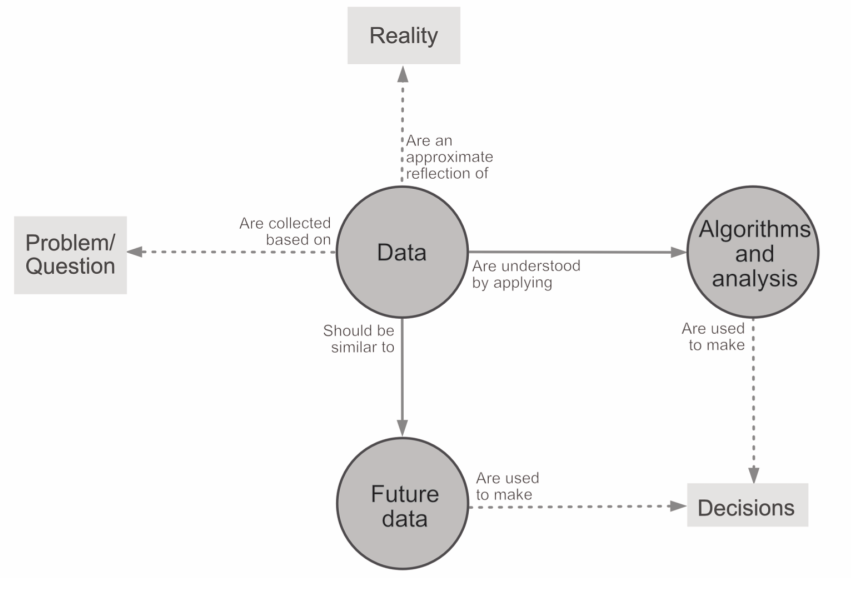
\includegraphics[width=\textwidth]{threerealms.png}
    \caption{Three realms of data science}
\end{figure}


\end{document}
